\chapter{Design}
%% TODO: the databases are selected considering: big data, scalability and data flexibility, different functionalities
The web application needs to handle a big amount of data, so we decided to use a combination of different databases to store and manage the data. 
We will use a document database to store users, media contents and reviews data, and a graph database to store relationships between users and media content. 
This will allow us to efficiently store and retrieve data, as well as handle complex relationships between data. 

\section{Document Database}
For the document database, we will use MongoDB. MongoDB is a NoSQL database that stores data in flexible, 
JSON-like documents. It is a popular choice for applications that require flexibility and scalability. 
These documents are 
flexible, meaning they can have different fields and structures. This makes MongoDB a good choice for 
applications that require flexibility in their data model. MongoDB is also a scalable database, meaning 
it can handle large amounts of data and traffic. It is designed to scale out, meaning you can add more 
servers to handle more traffic.
\newline
\newline
\textbf{Collections}
The database will have the following collections:
\begin{itemize}
    \item Anime: This collection will store information about anime, such as titles, tags, and synopsis.
    \item Manga: This collection will store information about manga, such as titles, genres, and authors.
    \item Reviews: This collection will store user ratings and comments for media content.
    \item Users: This collection will store user data, such as usernames, passwords, email addresses, gender and location.

\end{itemize}
\newpage
%% TODO: check the structure of the documents
\textbf{MongoDB document example}
\newline
Anime:
\begin{mdframed}[backgroundcolor=yellow!20, innerleftmargin=10pt, innerrightmargin=10pt]
    \begin{lstlisting}[language=java]
  {
  "_id": {
    "$oid": "65789bb52f5d29465d0abcfc"
  },
  "title": "\"Aesop\" no Ohanashi yori: Ushi to Kaeru, Yokubatta Inu",
  "type": "MOVIE",
  "episodes": 1,
  "status": "FINISHED",
  "picture": "https://cdn.myanimelist.net/images/anime/3/65151.jpg",
  "tags": [
    "family friendly",
    "fantasy",
    "frogs",
    "kids"
  ],
  "synopsis": "Based on Aesop's Fables.",
  "latest_reviews": [
    {
      "id": {
        "$oid": "657ed1b40481d3954cf8d69c"
      },
      "comment": "Struggles to maintain interest; fails to captivate.",
      "date": {
        "$date": "2022-04-11T22:00:00.000Z"
      },
      "user": {
        "id": {
          "$oid": "6577877ce683762347607f42"
        },
        "username": "dreadstuff",
        "picture": "https://imgbox.com/7MaTkBQR"
      }
    },
    {
      "id": {
        "$oid": "657ebc340481d3954cf842e5"
      },
      "comment": "Wouldn't recommend to even the most forgiving viewers.",
      "date": {
        "$date": "2021-03-19T23:00:00.000Z"
      },
      "user": {
        "id": {
          "$oid": "6577877ce683762347606bc6"
        },
        "username": "Yoma_Yuki",
        "picture": "https://imgbox.com/7MaTkBQR"
      }
    }
  ],
  "anime_season": {
    "season": "WINTER",
    "year": 1970
  },
  "average_rating": 4.5,
  "avg_rating_last_update": true,
  "review_ids": [
    "66695c50222b3184dbb7d990",
    "66695c50222b3184dbb7d991",
    "66695c50222b3184dbb7d992"
  ],
  "likes": 7
}
    \end{lstlisting}
\end{mdframed}

\newpage
Manga:
\begin{mdframed}[backgroundcolor=yellow!20, innerleftmargin=10pt, innerrightmargin=10pt]
    \begin{lstlisting}[language=java]
  {
    "_id": {
      "$oid": "657ac61cb34f5514b91eabc1"
    },
  "title": "H20",
  "type": "MANHWA",
  "status": "FINISHED",
  "volumes": 7,
  "chapters": 43,
  "genres": [
    "Romance",
    "Slice of Life"
  ],
  "demographics": [
    "SHOUJO"
  ],
  "authors": [
    {
      "id": 4354,
      "role": "Story & Art",
      "name": "Sook Ji Hwang"
    }
  ],
  "serializations": "Wink",
  "synopsis": "Menga is simply known as the vice rep and is bullied. Hanako has moved to Korea but was robbed the first day and has nothing. Na Hong Soo is known as a troublemaker and is in constant trouble. And Eechan is the student body president, very popular and known as Bacchus. It seems they have nothing in common but this will change soon. \n\n(Source: mangaupdates.com)",
  "title_english": "H20",
  "picture": "https://cdn.myanimelist.net/images/manga/1/1053l.jpg",
  "average_rating": 3.67,
  "latest_reviews": [
    {
      "id": {
        "$oid": "66682d94bebc20d9557bba39"
      },
      "comment": "Beautiful artwork and engaging characters.",
      "date": {
        "$date": "2024-06-17T21:33:37.000Z"
      },
      "rating": 7,
      "user": {
        "id": {
          "$oid": "6577877be68376234760635b"
        },
        "username": "Sanji-kun",
        "picture": "images/account-icon.png"
      }
    },
    {
      "id": {
        "$oid": "66682d94bebc20d9557bba35"
      },
      "comment": "An average manga with a few standout moments.",
      "date": {
        "$date": "2024-02-10T20:53:52.000Z"
      },
      "rating": 7,
      "user": {
        "id": {
          "$oid": "6577877ce6837623476065f0"
        },
        "username": "MangoSlushie",
        "picture": "https://thypix.com/wp-content/uploads/2021/10/manga-profile-picture-92.jpg"
      }
    }
  ],
  "start_date": null,
  "end_date": null,
  "avg_rating_last_update": true,
  "review_ids": [
    "66682d94bebc20d9557bba35",
    "66682d94bebc20d9557bba36",
    "66682d94bebc20d9557bba3b"
  ]
}
    \end{lstlisting}
\end{mdframed}


Reviews:
\begin{mdframed}[backgroundcolor=yellow!20, innerleftmargin=10pt, innerrightmargin=10pt]
    \begin{lstlisting}[language=java]
  {
  "_id": {
    "$oid": "66682a4fbebc20d9557b7542"
  },
  "user": {
    "id": {
      "$oid": "6577877ce683762347607b2f"
    },
    "username": "dagdffsfgf",
    "location": "Singapore",
    "birthday": {
      "$date": "1991-02-12T00:00:00.000Z"
    }
  },
  "manga": {
    "id": {
      "$oid": "657ac61bb34f5514b91ea22a"
    },
    "title": "Kaguya-sama wa Kokurasetai: Tensai-tachi no Renai Zunousen"
  },
  "rating": 9,
  "comment": "Rich in emotion and excitement.",
  "date": {
    "$date": "2022-07-18T07:18:21.000Z"
  }
} 
    \end{lstlisting}
\end{mdframed}

Users:
\begin{mdframed}[backgroundcolor=yellow!20, innerleftmargin=10pt, innerrightmargin=10pt]
    \begin{lstlisting}[language=java]
      {
  "_id": {
    "$oid": "6577877be683762347605859"
  },
  "email": "xdavis@example.com",
  "password": "290cb38a679d5eb68d11b9ea1e21f48234eba6de19f95612dbcb70ce0c7e4e78",
  "description": "Liberating the mind from stress with the power of anime zen.",
  "picture": "https://thypix.com/wp-content/uploads/2021/10/manga-profile-picture-44.jpg",
  "username": "Xinil",
  "gender": "Male",
  "birthday": {
    "$date": "1985-03-04T00:00:00.000Z"
  },
  "location": "South Africa",
  "joined_on": {
    "$date": "2016-11-30T00:00:00.000Z"
  },
  "app_rating": 1,
  "followed": 40,
  "followers": 29,
  "review_ids": [
    "66682a5cbebc20d9557b76b5",
    "66682b31bebc20d9557b8886",
    "66682e66bebc20d9557bcb29",
    "66683301bebc20d9557bf017"
  ]
}
    \end{lstlisting}
\end{mdframed}


The field \texttt{"app\_rating"} is used to know the general satisfaction of the user with the application.

\newpage

\subsection {CRUD operations}
\begin{itemize}
  %% TODO: specify all the crud operations
    \item Create: This operation will allow users to create new documents in the database. For example, users can create new reviews for anime and manga.
    \item Read: This operation will allow users to read documents from the database. For example, users can read information about anime and manga and about other users.
    \item Update: This operation will allow users to update documents in the database. For example, users can update their reviews for anime and manga, they can also update their own profile, the manager can update media contents.
    \item Delete: This operation will allow users to delete documents from the database. For example, users can delete their reviews for anime and manga, the manager can delete media contents.
\end{itemize}

\newpage
\section{Graph Database}
For the graph database, we will use Neo4j. Neo4j is a graph database that stores data in nodes and relationships. It is a popular choice for applications that require complex relationships between data. Neo4j is a graph database, which means it stores data in nodes and relationships. Nodes represent entities, such as users or products, and relationships represent connections between nodes. This makes Neo4j a good choice for applications that require complex relationships between data. Neo4j is also a scalable database, meaning it can handle large amounts of data and traffic. It is designed to scale out, meaning you can add more servers to handle more traffic. This makes Neo4j a good choice for applications that need to scale quickly.

\textbf{Nodes}

The database will have the following nodes:
\begin{itemize}
    \item User: This node will store information about users, such as id, usernames, and picture.
    \item Anime: This node will store information about anime, such as id, titles and picture.
    \item Manga: This node will store information about manga, such as id, titles and picture.
\end{itemize}

\textbf{Relationships}

The database will have the following relationships:
\begin{itemize}
    \item LIKE: This relationship will connect users to anime and manga nodes. It will store the date when the user liked the media content.
    \item FOLLOW: This relationship will connect users to other users. 
\end{itemize}

\begin{figure}[htbp]
    \centering
    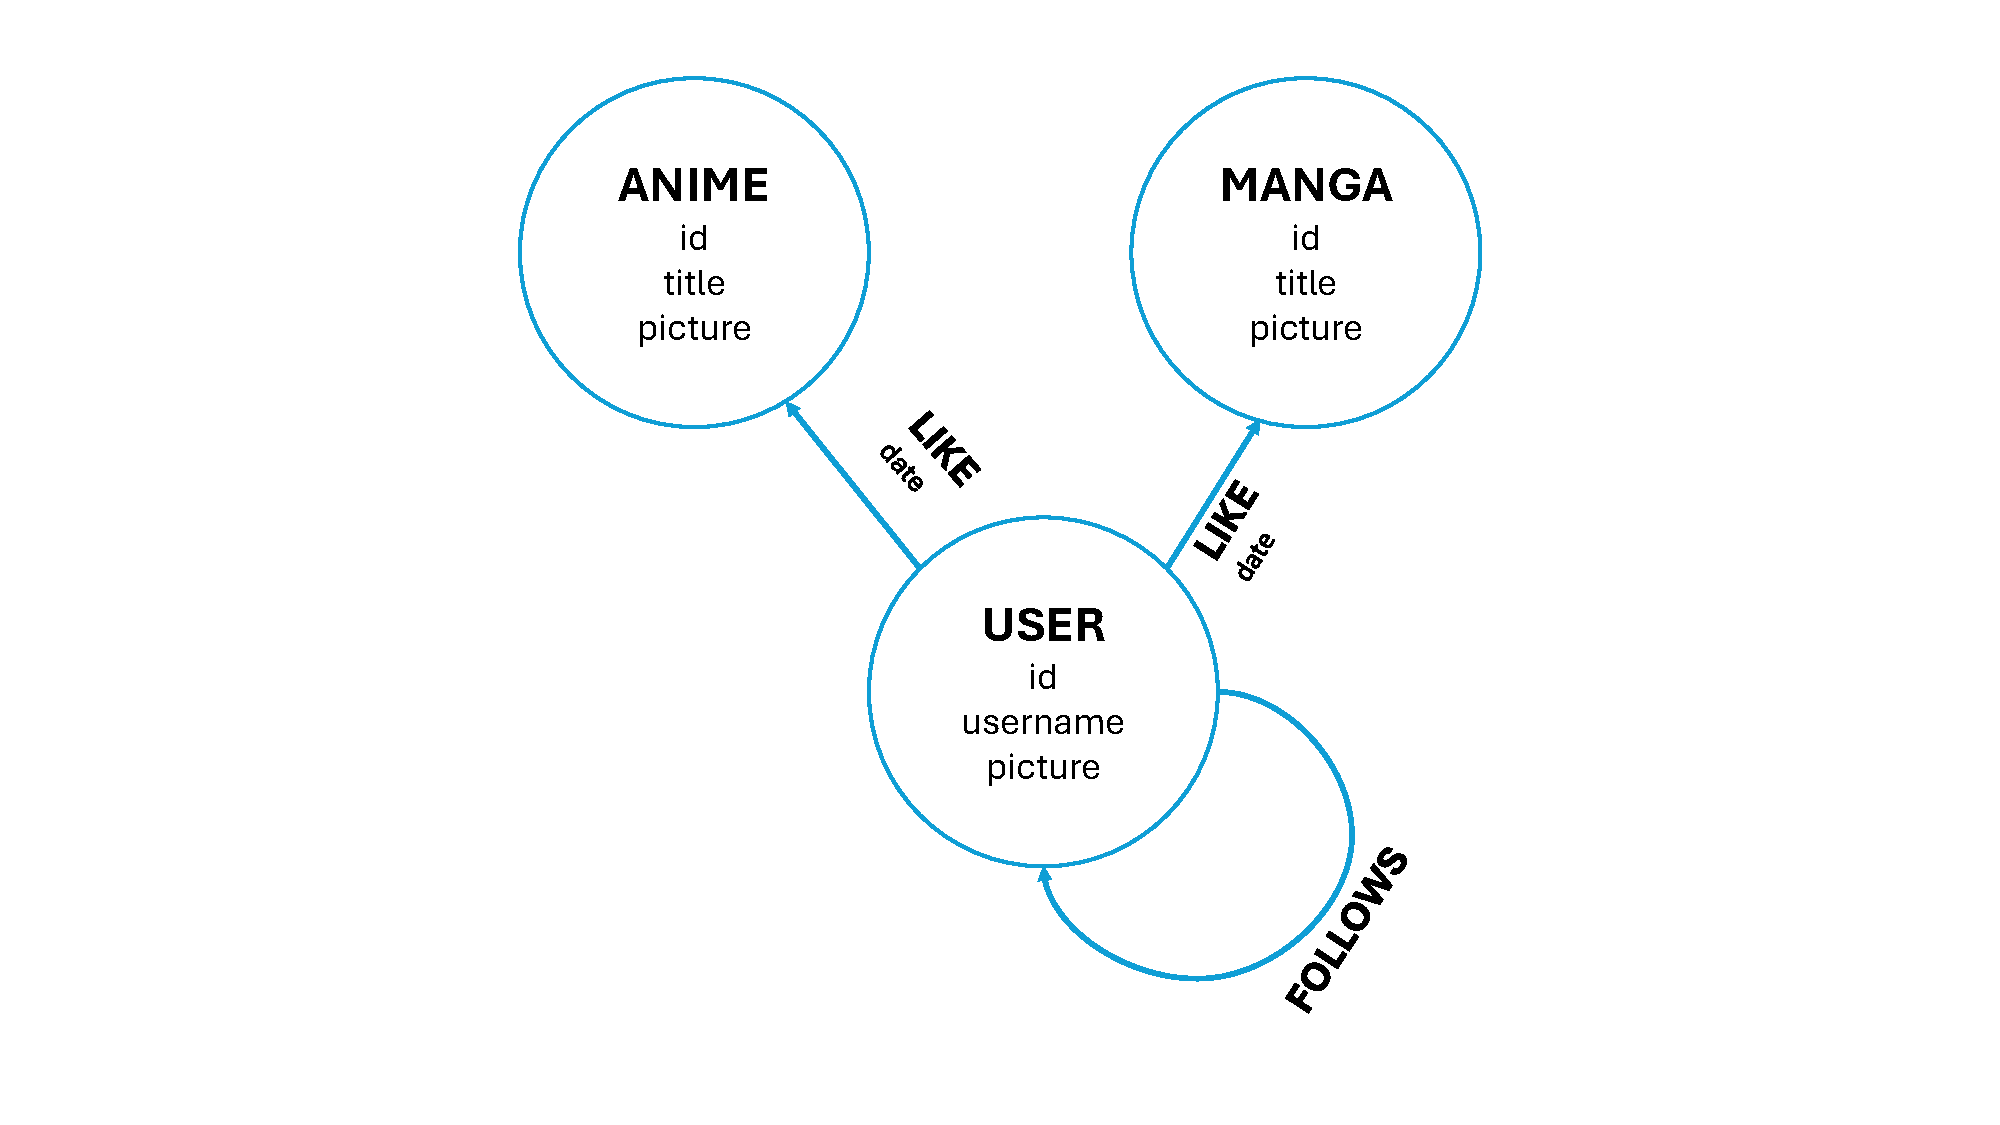
\includegraphics[width=\textwidth]{Media/graph.pdf}
    \caption{GraphDB}
    \label{fig:GraohDB}
\end{figure}

\newpage

\subsection{CRUD operations}
  %% TODO: specify all the crud operations

\begin{itemize}
    \item Create: This operation will allow users to create new nodes and relationships in the database. For example, users can create new relationships between users and media content:
    
    A user can LIKE a media content: 
    \begin{lstlisting}[language=Cypher, caption=Create Like Relationship]
    MATCH (u:User {id: $userId}), (a:Anime {id: $animeId}) 
    WHERE NOT (u)-[:LIKE]->(a) 
    CREATE (u)-[r:LIKE {date: $date} ]->(a)
    RETURN r
    \end{lstlisting}

    A user can FOLLOW another user:
    \begin{lstlisting}[language=Cypher, caption=Create Follow Relationship]
    MATCH (u:User {id: $userId}), (f:User {id: $followedUserId}) 
    WHERE NOT (u)-[:FOLLOWS]->(f) 
    CREATE (u)-[r:FOLLOWS]->(f) 
    RETURN r
    \end{lstlisting}

    \item Read: This operation will allow users to read nodes and relationships from the database. For example, users can read information about anime and manga and relationships between users and media content.
    A user can read the list of liked media contents:
    \begin{lstlisting}[language=Cypher, caption=Read Liked Media Contents]
  
    MATCH (u:User {id: $userId})-[:LIKE]->(a:Anime)
    RETURN a
    \end{lstlisting}

    A user can read the list of followers:
    \begin{lstlisting}[language=Cypher, caption=Read Followers]
    MATCH (u:User {id: $userId})<-[:FOLLOWS]-(f:User)
    RETURN f
    \end{lstlisting}
  
    \item Update: This operation will allow users to update nodes and relationships in the database. For example, users can update their likes for anime and manga and relationships between users.
    
    \item Delete: This operation will allow users to delete nodes and relationships from the database. For example, users can delete their likes for anime and manga and relationships between users.
    
    A user can unlike a media content:
    \begin{lstlisting}[language=Cypher, caption=Delete Like Relationship]
    MATCH (u:User {id: $userId})-[r:LIKE]->(a:Anime {id: $animeId})
    DELETE r
    RETURN r
    \end{lstlisting}
    \newpage
    A user can unfollow another user: 
    \begin{lstlisting}[language=Cypher, caption=Delete Follow Relationship]
    MATCH (:User {id: $followerUserId})-[r:FOLLOWS]->(:User {id: $followingUserId})
    DELETE r 
    RETURN r
    \end{lstlisting}
\end{itemize}

\section {Availability and Partition Tolerance}
MangaVerse, as a social network, gives priority to the AP configuration of the CAP theorem, ensuring Availability and Partition Tolerance. This allows users to access the application and interact with other users and media content, even if the data is not always consistent (Eventual Consistency).

\section{Redundancy}
%what is there to add here?
The performance of the application is critical, so we need to ensure that the system is highly available and fault-tolerant. To achieve this, we gave priority to fast responses, rather than reducing memory consumption.


\textbf{Latest reviews}


In the anime and manga collections, there's a field containing the latest 5 reviews written for that specific media content, in this way it's fast to retrieve. 


\textbf{Average rating}


In the anime and manga collections, there's a field containing the average rating of the media content, this field is updated every time a new review is written.


\textbf{Number of likes}


In the anime and manga collections, there's a field containing the number of likes, this field is updated every time a new like relationship is created or deleted.


\textbf{Followers and Followings}


In the user collection, there are fields containing the number of followers and followings, this field is updated every time a new follow relationship is created or deleted.


\textbf{User field in Reviews}


In the reviews collection, there's a field containing the user data, such as id, username, picture, and also location and birthday, which are used for suggestion porpouses.

\textbf{Media Content field in Reviews}


In the reviews collection, there's a field containg information about the anime or manga the reivew is about. This field has information about the media content id and title.


\textbf{Review Ids}


A list of review ids is stored in the anime, manga and users collections, this is used to quickly retrieve the reviews of a media content and of a user.

\section{Replicas}
A cluster of three nodes is available for this project, allowing deployment of replicas: however, replicas were only implemented in MongoDB, as Neo4j required the Enterprise version for it.
We have 3 replicas for MongoDB and 1 for Neo4J.
In MongoDB we have one primary and two secondary replicas, the primary is used for write operations and the secondaries are used for read operations. This will allow us to distribute the load and improve the performance of the application. In case of failure of the primary node, one of the secondary nodes will be promoted to primary, ensuring high availability of the system.

\newpage
\section{Sharding}
Sharding is a method for distributing data across multiple machines to meet the demands of data growth. As the size of the data increases, a single machine may not be sufficient to store the data nor provide an acceptable read and write throughput. Sharding typically solves the problem with horizontal scaling. However, in our application, sharding is not possible due to the nature of the collections and their interdependencies.

Our database consists of four collections: anime, manga, users, and reviews and each collection stores different types of information.
Sharding these collections would be complex due to their interrelated nature. The data in these collections is highly interconnected; for example, reviews reference both anime/manga and users, and each user can have multiple reviews linked to both anime and manga. Distributing such interdependent data across multiple shards would lead to significant overhead in maintaining relationships between documents, potentially causing performance degradation instead of improvement.

Therefore, while the database design is ready for sharding in theory, the practical constraints of our application's structure and the interconnectedness of our collections make sharding infeasible. Implementing sharding would introduce complexity and overhead that could outweigh the benefits of horizontal scaling in this context.

